\section{对数螺线}
\markboth{91. 对数螺线}{91. 对数螺线}

设 $e$ 是自然对数的底，$m$ 是不等于 $0$ 的常数，则极坐标方程
\[
  \rho = e^{m\theta}
\]
所表示的曲线叫做对数螺线，其形状如图 91.1 所示。

\begin{figure}[htbp]
  \centering
  \begin{tikzpicture}[scale=1.05]
    % 对数螺线 rho = R0 * exp(m*theta), theta in [-4*pi, 0.08*pi]
    \def\mval{0.22}
    \def\Rzero{1.15}
    \draw[line width=0.85pt, curveblue, domain=-12.56:0.25, samples=260, smooth]
      plot ({\Rzero*exp(\mval*\x)*cos(\x r)}, {\Rzero*exp(\mval*\x)*sin(\x r)});
    % 极轴 OP
    \draw[line width=0.65pt, -{Stealth[length=4.5pt]}] (0,0) -- (1.9,0);
    \fill (0,0) circle (1.2pt);
    \node[below=2pt] at (0,-0.02) {\footnotesize $O$};
    \node[below=2pt] at (1.82,-0.02) {\footnotesize $P$};
  \end{tikzpicture}
  \caption*{图\ 91.1}
\end{figure}

在自然界中，由于动、植物生长时细胞分裂的规律是一个变两个、两个变四个、四个变八个，等等，满足指数定律，因而在某些动物和植物身上可以找到自然存在的对数螺线。

\begin{figure}[htbp]
  \centering
  \begin{minipage}[b]{0.45\textwidth}
    \centering
    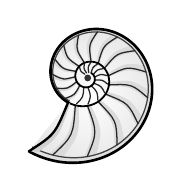
\begin{tikzpicture}[scale=1.08, line cap=round, line join=round]
      % 鹦鹉螺壳：顺时针向外盘旋，壳口自然朝右下方卧放，具双线外壳厚度、隔室弧线与天然条纹质感
      \def\bshell{0.175}
      \def\rshell{0.285}
      \def\phizero{0.78} % 使末端 t = 7.75 时极角 -(\phizero + t) 落在右下方约 -45°
      \def\tend{7.75}

      % 1) 壳体整体基底柔和渐变填充（摆脱单薄线框感）
      \pgfmathsetmacro{\tstart}{\tend - 6.28318}
      \pgfmathsetmacro{\reout}{\rshell*exp(\bshell*\tend)}
      \pgfmathsetmacro{\rein}{\rshell*exp(\bshell*\tstart)}
      \pgfmathsetmacro{\phiend}{-(\phizero + \tend)}
      \shade[inner color=white, outer color=black!9]
        plot[domain=\tstart:\tend, samples=160, smooth]
          ({\rshell*exp(\bshell*\x)*cos((-\phizero-\x) r)}, {\rshell*exp(\bshell*\x)*sin((-\phizero-\x) r)})
        -- ({\rein*cos(\phiend r)}, {\rein*sin(\phiend r)}) -- cycle;

      % 2) 外圈隔室天然条纹与明暗过渡（外缘略深、近壳脐渐淡）
      \foreach \th in {1.50, 1.92, ..., 7.45} {
        \pgfmathsetmacro{\tha}{\th}
        \pgfmathsetmacro{\thb}{\th + 0.16}
        \pgfmathsetmacro{\roA}{0.94*\rshell*exp(\bshell*\tha)}
        \pgfmathsetmacro{\roB}{0.94*\rshell*exp(\bshell*\thb)}
        \pgfmathsetmacro{\riA}{\rshell*exp(\bshell*(\tha-6.28318))}
        \pgfmathsetmacro{\riB}{\rshell*exp(\bshell*(\thb-6.28318))}
        \pgfmathsetmacro{\pA}{-(\phizero + \tha)}
        \pgfmathsetmacro{\pB}{-(\phizero + \thb)}
        \pgfmathsetmacro{\rmA}{0.52*(\roA+\riA)}
        \pgfmathsetmacro{\rmB}{0.52*(\roB+\riB)}
        \fill[black!14]
          ({\riA*cos(\pA r)}, {\riA*sin(\pA r)})
          .. controls ({\rmA*cos((\pA+0.16) r)}, {\rmA*sin((\pA+0.16) r)}) ..
          ({\roA*cos(\pA r)}, {\roA*sin(\pA r)})
          -- ({\roB*cos(\pB r)}, {\roB*sin(\pB r)})
          .. controls ({\rmB*cos((\pB+0.16) r)}, {\rmB*sin((\pB+0.16) r)}) ..
          ({\riB*cos(\pB r)}, {\riB*sin(\pB r)}) -- cycle;
      }

      % 3) 双线外壳壁厚度填充与内壁细线
      \fill[black!12]
        plot[domain=1.46:\tend, samples=150, smooth]
          ({\rshell*exp(\bshell*\x)*cos((-\phizero-\x) r)}, {\rshell*exp(\bshell*\x)*sin((-\phizero-\x) r)})
        -- plot[domain=\tend:1.46, samples=150, smooth]
          ({0.94*\rshell*exp(\bshell*\x)*cos((-\phizero-\x) r)}, {0.94*\rshell*exp(\bshell*\x)*sin((-\phizero-\x) r)})
        -- cycle;
      \draw[line width=0.45pt, black!75, domain=1.46:\tend, samples=160, smooth]
        plot ({0.94*\rshell*exp(\bshell*\x)*cos((-\phizero-\x) r)}, {0.94*\rshell*exp(\bshell*\x)*sin((-\phizero-\x) r)});

      % 4) 隔室弧线（沿生长反方向内凹的优雅隔膜线）
      \foreach \th in {-3.0, -2.58, ..., 7.55} {
        \pgfmathsetmacro{\rout}{0.94*\rshell*exp(\bshell*\th)}
        \pgfmathsetmacro{\rin}{\rshell*exp(\bshell*(\th-6.28318))}
        \pgfmathsetmacro{\rmid}{0.52*(\rout+\rin)}
        \pgfmathsetmacro{\p}{-(\phizero + \th)}
        \pgfmathsetmacro{\pmid}{\p + 0.18}
        \draw[line width=0.46pt, black!85]
          ({\rin*cos(\p r)}, {\rin*sin(\p r)})
          .. controls ({\rmid*cos(\pmid r)}, {\rmid*sin(\pmid r)}) ..
          ({\rout*cos(\p r)}, {\rout*sin(\p r)});
      }

      % 5) 内部中心旋涡与深色壳脐
      \draw[line width=0.65pt, domain=-8.0:1.46, samples=140, smooth]
        plot ({\rshell*exp(\bshell*\x)*cos((-\phizero-\x) r)}, {\rshell*exp(\bshell*\x)*sin((-\phizero-\x) r)});
      \fill[black!80] (0,0) circle (0.04);

      % 6) 外廓主螺线与右下方微凹壳口闭合线（附内侧轻阴影）
      \draw[line width=0.95pt, black, domain=1.46:\tend, samples=180, smooth]
        plot ({\rshell*exp(\bshell*\x)*cos((-\phizero-\x) r)}, {\rshell*exp(\bshell*\x)*sin((-\phizero-\x) r)});
      \pgfmathsetmacro{\rmend}{0.52*(\reout+\rein)}
      \fill[black!18]
        ({\rein*cos(\phiend r)}, {\rein*sin(\phiend r)})
        .. controls ({\rmend*cos((\phiend+0.15) r)}, {\rmend*sin((\phiend+0.15) r)}) ..
        ({\reout*cos(\phiend r)}, {\reout*sin(\phiend r)})
        -- ({0.94*\reout*cos((\phiend+0.09) r)}, {0.94*\reout*sin((\phiend+0.09) r)})
        .. controls ({\rmend*cos((\phiend+0.22) r)}, {\rmend*sin((\phiend+0.22) r)}) ..
        ({\rein*cos((\phiend+0.08) r)}, {\rein*sin((\phiend+0.08) r)}) -- cycle;
      \draw[line width=0.85pt, black]
        ({\rein*cos(\phiend r)}, {\rein*sin(\phiend r)})
        .. controls ({\rmend*cos((\phiend+0.15) r)}, {\rmend*sin((\phiend+0.15) r)}) ..
        ({\reout*cos(\phiend r)}, {\reout*sin(\phiend r)});
    \end{tikzpicture}
    \caption*{图\ 91.2}
  \end{minipage}
  \hfill
  \begin{minipage}[b]{0.50\textwidth}
    \centering
    \begin{tikzpicture}[scale=0.96, line cap=round, line join=round]
      % 重瓣花朵：严格按黄金角 137.507764 度与指数半径 R_j = 0.22 * exp(0.033*j) 排布饱满花瓣
      % 从外向内 (j = 54 down to 0) 绘制并带柔和底影，自然形成层叠立体感
      \def\Rzero{0.22}
      \def\cval{0.033}
      \foreach \j in {54,53,...,0} {
        \pgfmathsetmacro{\ang}{\j * 137.507764}
        \pgfmathsetmacro{\rTip}{\Rzero * exp(\cval * \j)}
        \pgfmathsetmacro{\rBase}{0.36 * \rTip}
        \pgfmathsetmacro{\plen}{\rTip - \rBase}
        \pgfmathsetmacro{\pwid}{0.48 * \plen + 0.055}
        \begin{scope}[rotate=\ang]
          \path[draw=black, line width=0.52pt, top color=white, bottom color=black!7]
            (0,\rBase)
            .. controls (-\pwid,{\rBase + 0.42*\plen}) and ({-\pwid*0.92},{\rTip - 0.14*\plen}) ..
            (0,\rTip)
            .. controls ({\pwid*0.92},{\rTip - 0.14*\plen}) and (\pwid,{\rBase + 0.42*\plen}) ..
            (0,\rBase) -- cycle;
          \draw[line width=0.22pt, black!48] (0,{\rBase + 0.14*\plen}) -- (0,{\rTip - 0.24*\plen});
        \end{scope}
      }
      % 花心小蕊
      \fill[white, draw=black, line width=0.5pt] (0,0) circle (0.095);
      \foreach \a in {0,45,...,315} {
        \fill (\a:0.048) circle (0.42pt);
      }
      % 两条严格串过花瓣尖端的虚线对数螺线（因花瓣尖端在 (0, rTip) 旋转 \ang 度，极角须补加 +90 度）
      % 1) 8-斜列线 (逆时针, j = 2 + 8*t): 先绘轻微白边衬底，再绘深色加粗长虚线
      \draw[line width=2.2pt, white, opacity=0.82,
            domain=0:6.2, samples=90, smooth]
        plot ({ \Rzero*exp(\cval*(2 + 8*\x)) * cos( (2*137.507764 + \x*20.062112 + 90) ) },
              { \Rzero*exp(\cval*(2 + 8*\x)) * sin( (2*137.507764 + \x*20.062112 + 90) ) });
      \draw[dashed, dash pattern=on 3.8pt off 2.2pt, line width=1.15pt, curveblue!85!black,
            domain=0:6.2, samples=90, smooth]
        plot ({ \Rzero*exp(\cval*(2 + 8*\x)) * cos( (2*137.507764 + \x*20.062112 + 90) ) },
              { \Rzero*exp(\cval*(2 + 8*\x)) * sin( (2*137.507764 + \x*20.062112 + 90) ) });
      % 2) 5-斜列线 (顺时针, j = 4 + 5*t): 同样白边衬底 + 深色加粗长虚线
      \draw[line width=2.2pt, white, opacity=0.82,
            domain=0:10.0, samples=110, smooth]
        plot ({ \Rzero*exp(\cval*(4 + 5*\x)) * cos( (4*137.507764 - \x*32.461180 + 90) ) },
              { \Rzero*exp(\cval*(4 + 5*\x)) * sin( (4*137.507764 - \x*32.461180 + 90) ) });
      \draw[dashed, dash pattern=on 3.8pt off 2.2pt, line width=1.15pt, curveblue!85!black,
            domain=0:10.0, samples=110, smooth]
        plot ({ \Rzero*exp(\cval*(4 + 5*\x)) * cos( (4*137.507764 - \x*32.461180 + 90) ) },
              { \Rzero*exp(\cval*(4 + 5*\x)) * sin( (4*137.507764 - \x*32.461180 + 90) ) });
    \end{tikzpicture}
    \caption*{图\ 91.3}
  \end{minipage}
\end{figure}

例如，图 91.2 所示的螺壳，明显地呈现对数螺线形状。在图 91.3 所示的花朵中，也可看出花瓣沿着对数螺线排列（图中用虚线画出两条对数螺线）。如果仔细观察向日葵的花盘，还会发现一粒一粒的葵花籽在花盘上也是排成很多条交织的对数螺线。

对数螺线的方程还可写成其它形式。例如记 $e^m = a$，就能把对数螺线方程改写成最简洁的形式
\[
  \rho = a^\theta.
\]

另一方面，如果把极轴旋转一个任意的角 $\alpha$，那么点 $(\rho, \theta)$ 的极坐标变成 $(\rho, \theta_1)$，这里 $\theta_1 = \theta - \alpha$，因而原方程 $\rho = e^{m\theta}$ 变成
\[
  \rho = e^{m(\theta_1 + \alpha)}.
\]
记 $m\alpha = b + \ln C$，并且略去 $\theta$ 的下标 $1$，上式就化为
\[
  \rho = C e^{m\theta + b},
\]
这是对数螺线方程的最一般的形式。
